\section{Modelo conceptual}
\begin{landscape}
\subsection{Diagrama}
\begin{figure}[H]
\centering
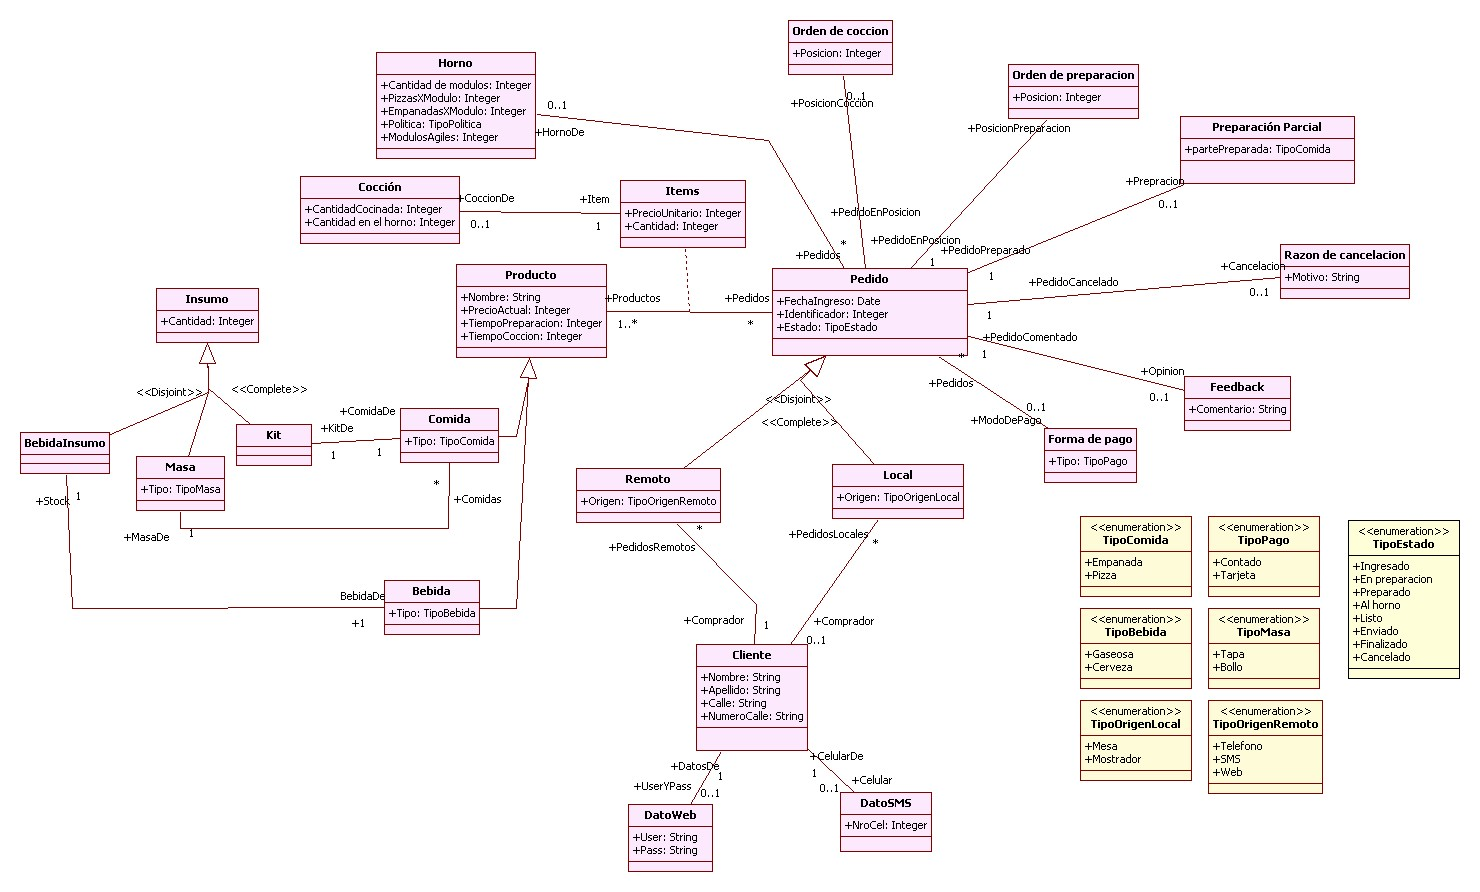
\includegraphics[height=16cm]{conceptos}
\end{figure}
\end{landscape}
En el diagrama lo que observamos primeramente es que los pedidos son el concepto principal. Un pedido tiene una fecha de ingreso, un identificador unico en el sistema, y un estado. El pedido esta asociado a varios productos (Pizzas de muzzarella, napolitana, empanadas de carne, coca cola), y lleva una cierta cantidad de cada uno de ellos. Ademas estos productos se ligaron al pedido con un precio particular, que no necesariamente es el precio actual ya que los precios pueden cambiar.
Segun el estado que posea un pedido, esta relacionado con diferentes clases conceptuales
\subsection{Diccionario de datos} %TODO: no se q es

\subsection{Restricciones al MC en OCL}
\restr{Un pedido tiene un conjunto de estados valido}{}
\restr{Un pedido llega a los estado en orden valido}{}
\restr{Si el pedido no era en el local o ya fue entregado, entonces tiene una forma de pago}{}
\restr{Forma de pago tarjeta si y solo si pedido local o web}{}
\restr{Cliente tiene pedidos remotos web si tiene datos web y remotos sms si tiene numero de celular}{}
\restr{Si el pedido tiene solo pizzas y se esta preparando, empanadaspreparadas es true}{}
\restr{Si el pedido tiene solo empanadas y se esta preparando, pizzaspreparadas es true}{}
\restr{Un pedido tiene feedback si era remoto}{}
\restr{Cada estado se relaciona con un estado-pedido adecuado}{}
\restr{Todos los datos web son diferentes}{}
%TODO: q onda con los numeros?
\restr{Todos los numeros de celular son diferentes}{}
\restr{Todos los numeros de telefono son diferentes}{}
%TODO: dudoso
\restr{Para los pedidos de la misma fecha, los precios de sus items son iguales}{}
\restr{Un pedido tiene un horno si y solo si no es de solo bebidas}{}
\restr{Hay solo siete estados y tienen los nombres de los estados de pedido}{}
\restr{No hay dos pedidos con el mismo identificador}{}
\restr{}{}